\newpage
\section{3次元ダムブレイク}
二層流のベンチマーク問題として3次元のダムブレイク問題を解析した。

\subsection{解析条件}

Table \ref{table:dambreak-material-property}に二つの流体の物性値を示す。
Case1は水と空気の物性値である。
\renewcommand{\arraystretch}{1}
\begin{table}[H]
	\centering
	\caption{物性値}
	\begin{tabular}{ccccccc}
		\hline
		Test case & $\rho_1 (\mathrm{kg/m^3})$ & $\rho_2 (\mathrm{kg/m^3})$ & $\mu_1 (\mathrm{Ns/m^2})$& $\mu_2 (\mathrm{Ns/m^2})$ & $\mathrm{g} (\mathrm{m/s^2})$ \\
		\hline 
		Case$1$ & $998$ & $1.205$   & $1.01\times10^{-3}$ & $1.81\times10^{-5}$ & $9.81$ \\
		\hline         
	\end{tabular}
	\label{table:dambreak-material-property}
\end{table}
\renewcommand{\arraystretch}{1.0}

代表長さ$a=0.146 \mathrm{m}$として、
水柱の初期高さ$a(=0.146\mathrm{m})$、初期幅$2a(=0.292\mathrm{m})$、領域の高さ$2.4a(=0.3504\mathrm{m})$、幅$4a(=0.584\mathrm{m})$、奥行き$0.1a(=0.0146\mathrm{m})$とした。

\begin{figure}[H]
	\centering
	\includegraphics[width=10truecm]{pics/3d-dambreak/dambreak_geometry.png}
	\caption{領域の寸法\cite{Koshizuka1996}}
	\label{fig:3d-dambreak-geometry}
\end{figure}


Table \ref{table:dambreak-parameter}に解析における設定パラメータを示す。
界面幅$D$は、近似ヘビサイド関数よる平滑化の計算式(\ref{ls-heaviside})に含まれるパラメータである。
Case1と2では$D$の値が異なり、Case2の方がCase1よりも界面が平滑化される。
\renewcommand{\arraystretch}{1}
\begin{table}[H]
	\centering
	\caption{解析パラメータ}
	\begin{tabular}{cccccc}
		\hline
		Test case & $\Delta t$ & メッシュ幅$dx$ & 界面幅$D$ & 再初期化回数 & 再初期化$\Delta \tau$\\
		\hline 
		Case$1$ & $0.00025$ & $0.0146$ & $0.0438$ & $5$ & $0.0001$\\
		\hline         
	\end{tabular}
	\label{table:dambreak-parameter}
\end{table}
\renewcommand{\arraystretch}{1.0}

Figure \ref{fig:3d-dambreak-mesh}に解析用のメッシュを示す。メッシュは六面体$1$次要素を使用した。
Figure \ref{fig:3d-dambreak-boundary}に初期状態のレベルセット関数と、境界条件を示す。

\begin{figure}[H]
	\centering
	\begin{minipage}[b]{0.49\columnwidth}
	    \centering
		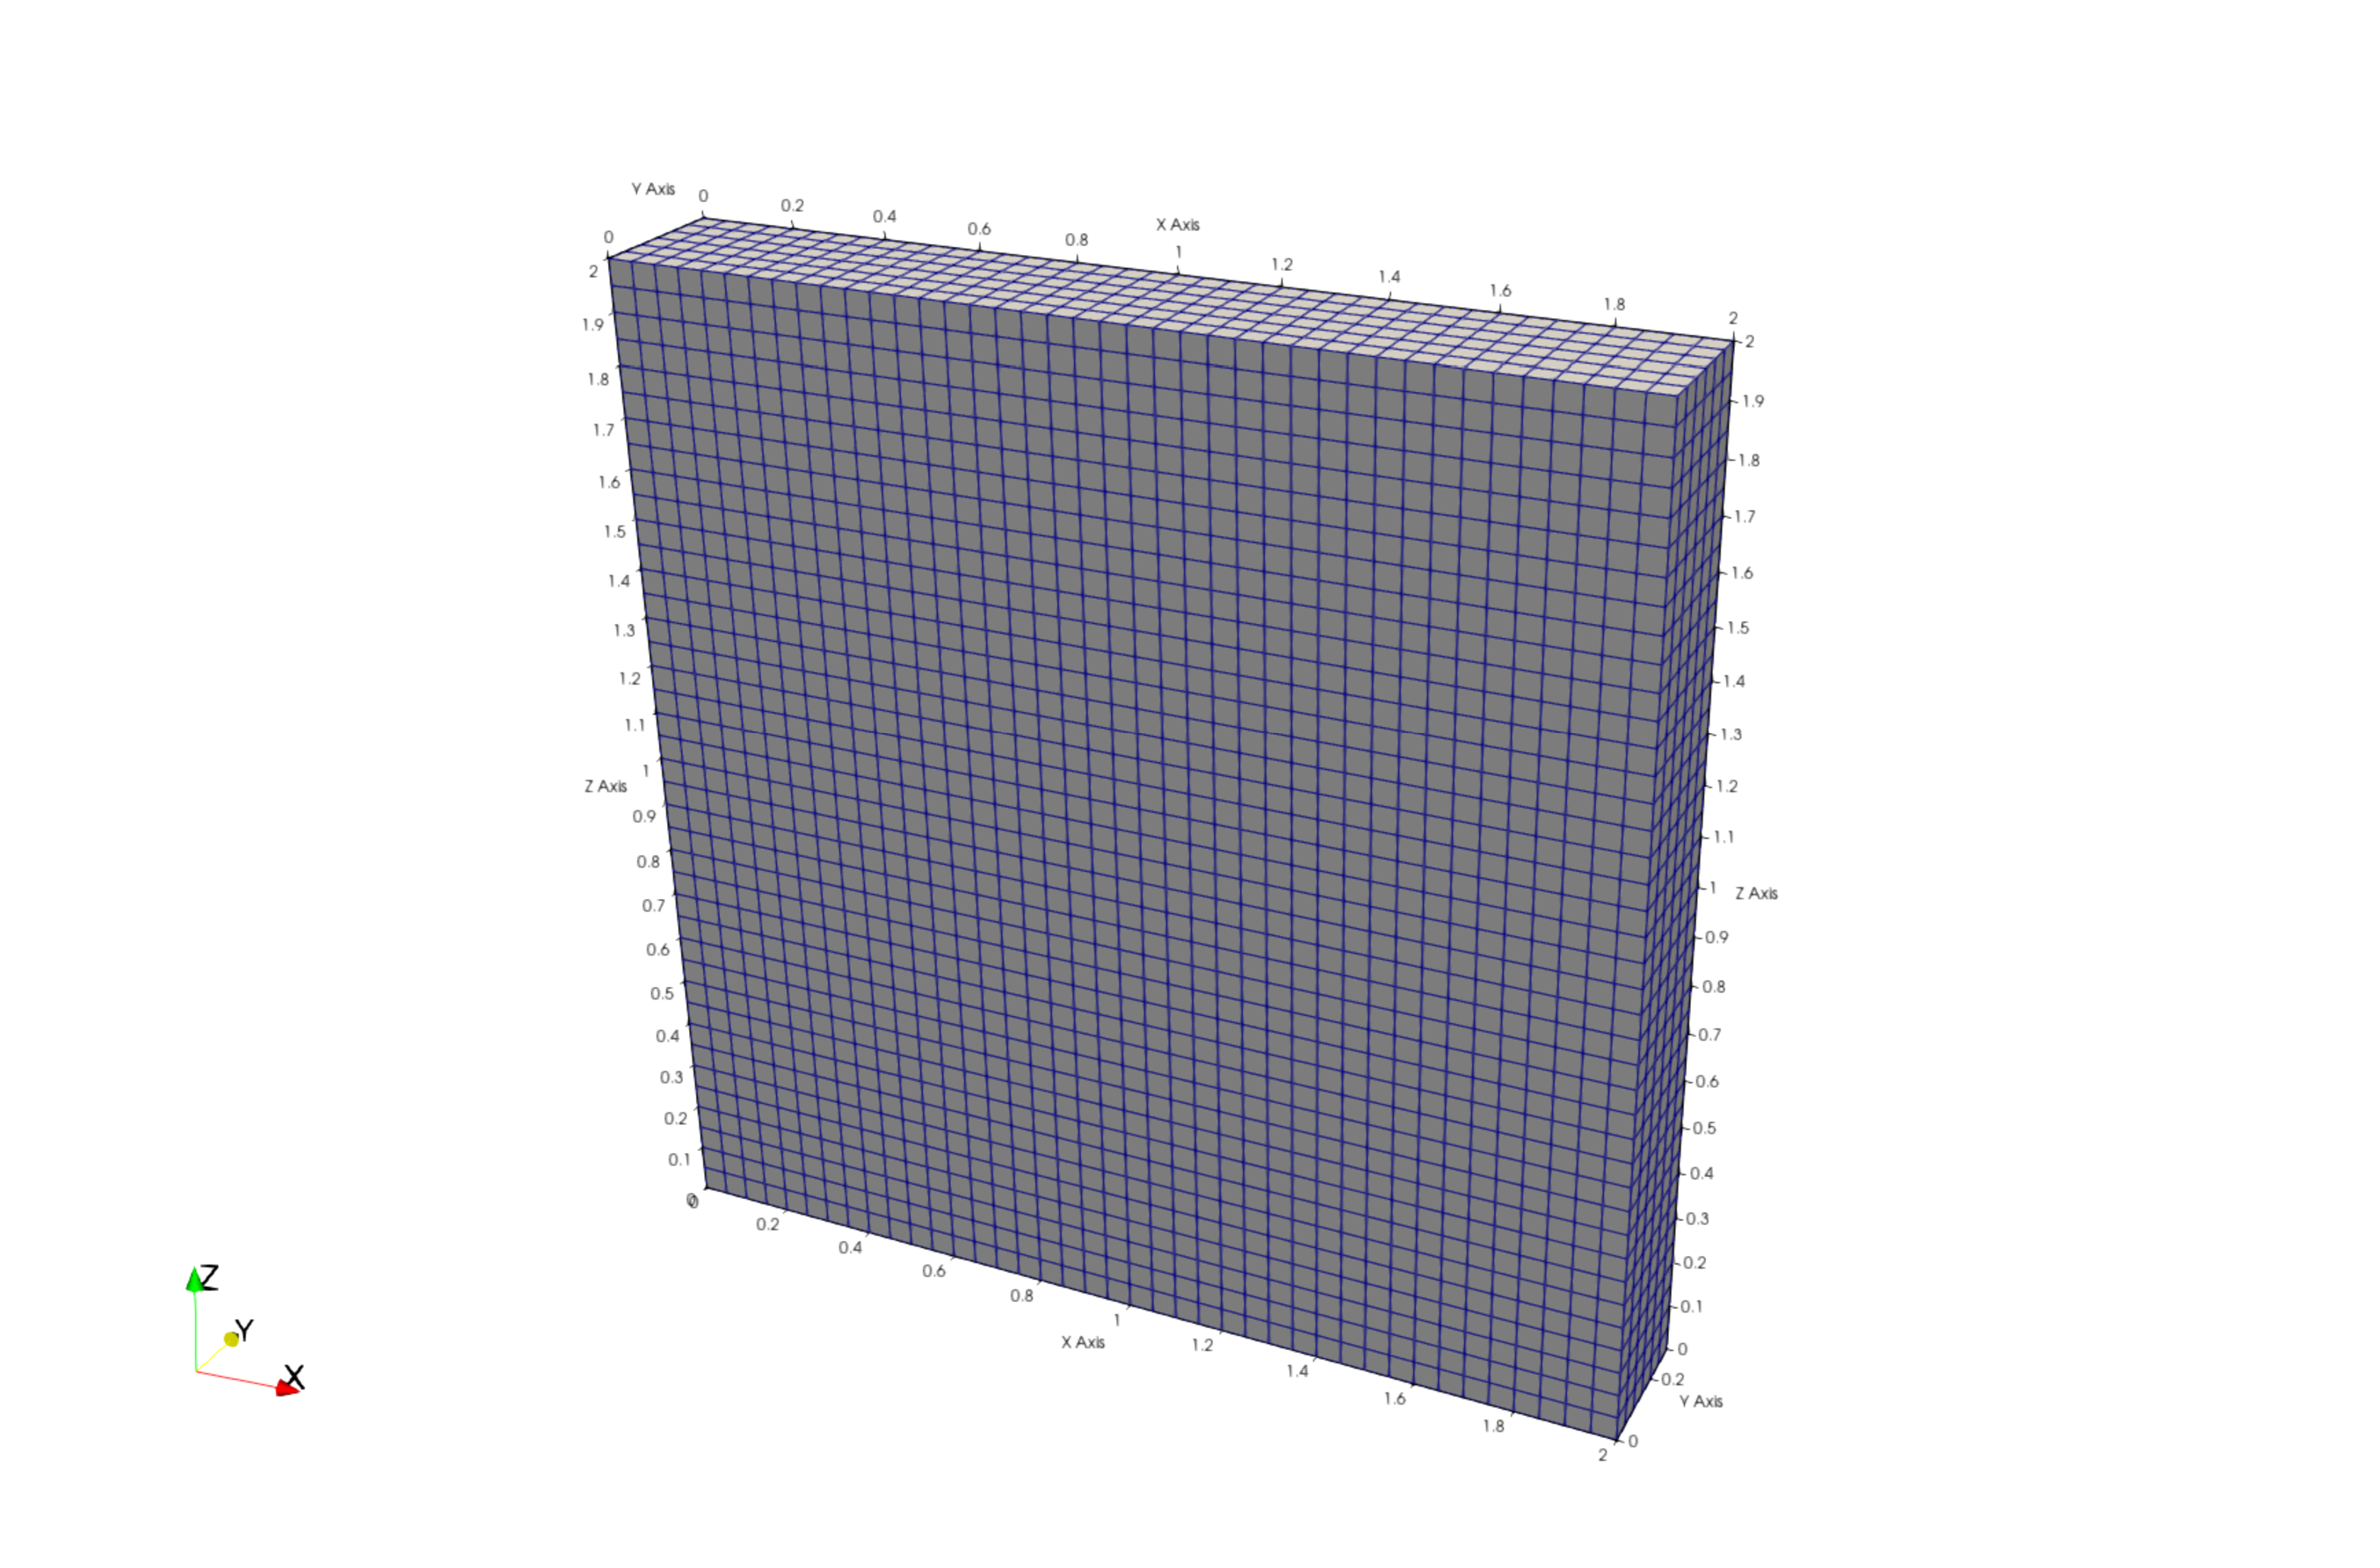
\includegraphics[width=10truecm]{pics/3d-dambreak-parallel/mesh.jpeg}
		\caption{ダムブレイクの計算メッシュ}
		\label{fig:3d-dambreak-mesh}
	\end{minipage}
	\begin{minipage}[b]{0.49\columnwidth}
	    \centering
		\includegraphics[width=10truecm]{pics/3d-dambreak-parallel/heaviside_init.jpeg}
		\caption{ダムブレイクの初期のレベルセット関数と境界条件。全面slip条件}
		\label{fig:3d-dambreak-boundary}
	\end{minipage}
\end{figure}

\subsection{解析結果}

\begin{figure}[H]
	\centering
	\begin{minipage}[b]{0.19\columnwidth}
	    \centering
	    \includegraphics[width=3.5truecm]{pics/3d-dambreak/result_0000.jpeg}
	\end{minipage}
	\begin{minipage}[b]{0.19\columnwidth}
	    \centering
	    \includegraphics[width=3.5truecm]{pics/3d-dambreak/result_0010.jpeg}
	\end{minipage}
	\begin{minipage}[b]{0.19\columnwidth}
	    \centering
	    \includegraphics[width=3.5truecm]{pics/3d-dambreak/result_0020.jpeg}
	\end{minipage}
	\begin{minipage}[b]{0.19\columnwidth}
	    \centering
	    \includegraphics[width=3.5truecm]{pics/3d-dambreak/result_0030.jpeg}
	\end{minipage}
	\begin{minipage}[b]{0.19\columnwidth}
	    \centering
	    \includegraphics[width=3.5truecm]{pics/3d-dambreak/result_0040.jpeg}
	\end{minipage}

	\caption{ダムブレイクの結果}
	\label{fig:dambreak-result}
\end{figure}

\begin{figure}[H]
	\centering
	\begin{minipage}[b]{0.19\columnwidth}
	    \centering
	    \includegraphics[width=3.5truecm]{pics/3d-dambreak/result_0050.jpeg}
	\end{minipage}
	\begin{minipage}[b]{0.19\columnwidth}
	    \centering
	    \includegraphics[width=3.5truecm]{pics/3d-dambreak/result_0060.jpeg}
	\end{minipage}
	\begin{minipage}[b]{0.19\columnwidth}
	    \centering
	    \includegraphics[width=3.5truecm]{pics/3d-dambreak/result_0070.jpeg}
	\end{minipage}
	\begin{minipage}[b]{0.19\columnwidth}
	    \centering
	    \includegraphics[width=3.5truecm]{pics/3d-dambreak/result_0080.jpeg}
	\end{minipage}
	\begin{minipage}[b]{0.19\columnwidth}
	    \centering
	    \includegraphics[width=3.5truecm]{pics/3d-dambreak/result_0090.jpeg}
	\end{minipage}

	\caption{ダムブレイクの結果}
	\label{fig:dambreak-result}
\end{figure}

\begin{figure}[H]
	\centering
	\includegraphics[width=10truecm]{pics/3d-dambreak/dambreak_result_v_and_v.pdf}
	\caption{Referenceとの比較\cite{Martin1952}}
	\label{fig:3d-dambreak-result-comparison}
\end{figure}

\begin{comment}
\begin{figure}[H]
	\centering
	\includegraphics[width=4truecm]{pics/3d-dambreak/experiment_koshizuka1996.png}
	\caption{Referenceとの比較\cite{Koshizuka1996}}
	\label{fig:3d-dambreak-result-picture}
\end{figure}

\begin{comment}
\subsection{体積保存を入れない場合の結果}

\begin{figure}[H]
	\centering
	\begin{minipage}[b]{0.19\columnwidth}
	    \centering
	    \includegraphics[width=3.5truecm]{pics/3d-dambreak/no_volume_correction/result_0000.jpeg}
	\end{minipage}
	\begin{minipage}[b]{0.19\columnwidth}
	    \centering
	    \includegraphics[width=3.5truecm]{pics/3d-dambreak/no_volume_correction/result_0010.jpeg}
	\end{minipage}
	\begin{minipage}[b]{0.19\columnwidth}
	    \centering
	    \includegraphics[width=3.5truecm]{pics/3d-dambreak/no_volume_correction/result_0020.jpeg}
	\end{minipage}
	\begin{minipage}[b]{0.19\columnwidth}
	    \centering
	    \includegraphics[width=3.5truecm]{pics/3d-dambreak/no_volume_correction/result_0030.jpeg}
	\end{minipage}
	\begin{minipage}[b]{0.19\columnwidth}
	    \centering
	    \includegraphics[width=3.5truecm]{pics/3d-dambreak/no_volume_correction/result_0033.jpeg}
	\end{minipage}

	\caption{ダムブレイクの結果(体積保存を入れない場合)}
	\label{fig:dambreak-result}
\end{figure}


\subsection{レベルセット関数の最初期化を入れない場合の結果}

\begin{figure}[H]
	\centering
	\begin{minipage}[b]{0.19\columnwidth}
	    \centering
	    \includegraphics[width=3.5truecm]{pics/3d-dambreak/no_reinitialization/result_0000.jpeg}
	\end{minipage}
	\begin{minipage}[b]{0.19\columnwidth}
	    \centering
	    \includegraphics[width=3.5truecm]{pics/3d-dambreak/no_reinitialization/result_0010.jpeg}
	\end{minipage}
	\begin{minipage}[b]{0.19\columnwidth}
	    \centering
	    \includegraphics[width=3.5truecm]{pics/3d-dambreak/no_reinitialization/result_0020.jpeg}
	\end{minipage}
	\begin{minipage}[b]{0.19\columnwidth}
	    \centering
	    \includegraphics[width=3.5truecm]{pics/3d-dambreak/no_reinitialization/result_0030.jpeg}
	\end{minipage}
	\begin{minipage}[b]{0.19\columnwidth}
	    \centering
	    \includegraphics[width=3.5truecm]{pics/3d-dambreak/no_reinitialization/result_0040.jpeg}
	\end{minipage}

	\caption{ダムブレイクの結果(再初期化を入れない場合)}
	\label{fig:dambreak-result}
\end{figure}
\end{comment}

\subsection{参考:高粘性流体のケース(コンクリートのビンガム流体を想定した事前検討)}
今後ビンガム流体による解析を取り入れるにあたって、高粘性流体でも安定的に解析できるかどうかを事前検討として確認した。
コンクリートの物性値は文献\cite{Saito2012}より、密度$\rho=3000\mathrm{kg/m^3}$、粘性係数は$\mu = 1 \mathrm{kg/(m\cdot s)}$と$\mu=1000 \mathrm{kg/(m\cdot s)}$の2パターンで確認した。
どちらのケースでも水と空気のダムブレイクから物性値だけを変えた解析条件で安定に解析できたため、ビンガム流体に変更したときも不安定性が出る可能性は低いと考えられる。

図\ref{fig:dambreak-result-visc1-1}と\ref{fig:dambreak-result-visc1-2}に$\mu = 1 \mathrm{kg/(m\cdot s)}$のケースの結果を、
図\ref{fig:dambreak-result-visc1000-1}と\ref{fig:dambreak-result-visc1000-2}に$\mu = 1000 \mathrm{kg/(m\cdot s)}$のケースの結果を示す。

図\ref{fig:3d-dambreak-concrete-reference}のビンガム流体の計算の参考文献の結果\cite{Saito2012}と比較すると、$\mu = 1000 \mathrm{kg/(m\cdot s)}$のケースの結果が近い動きをしており、ビンガム流体の計算の事前検討としては近い条件を模擬できていると考えられる。

\begin{figure}[H]
	\centering
	\begin{minipage}[b]{0.19\columnwidth}
	    \centering
	    \includegraphics[width=3.5truecm]{pics/3d-dambreak/viscosity1/result_0000.jpeg}
	\end{minipage}
	\begin{minipage}[b]{0.19\columnwidth}
	    \centering
	    \includegraphics[width=3.5truecm]{pics/3d-dambreak/viscosity1/result_0010.jpeg}
	\end{minipage}
	\begin{minipage}[b]{0.19\columnwidth}
	    \centering
	    \includegraphics[width=3.5truecm]{pics/3d-dambreak/viscosity1/result_0020.jpeg}
	\end{minipage}
	\begin{minipage}[b]{0.19\columnwidth}
	    \centering
	    \includegraphics[width=3.5truecm]{pics/3d-dambreak/viscosity1/result_0030.jpeg}
	\end{minipage}
	\begin{minipage}[b]{0.19\columnwidth}
	    \centering
	    \includegraphics[width=3.5truecm]{pics/3d-dambreak/viscosity1/result_0040.jpeg}
	\end{minipage}
	\caption{ダムブレイクの結果(粘性係数$\mu = 1 \mathrm{kg/(m\cdot s)}$, $T=0 \sim 40$)}
	\label{fig:dambreak-result-visc1-1}
\end{figure}

\begin{figure}[H]
	\centering
	\begin{minipage}[b]{0.19\columnwidth}
	    \centering
	    \includegraphics[width=3.5truecm]{pics/3d-dambreak/viscosity1/result_0050.jpeg}
	\end{minipage}
	\begin{minipage}[b]{0.19\columnwidth}
	    \centering
	    \includegraphics[width=3.5truecm]{pics/3d-dambreak/viscosity1/result_0060.jpeg}
	\end{minipage}
	\begin{minipage}[b]{0.19\columnwidth}
	    \centering
	    \includegraphics[width=3.5truecm]{pics/3d-dambreak/viscosity1/result_0070.jpeg}
	\end{minipage}
	\begin{minipage}[b]{0.19\columnwidth}
	    \centering
	    \includegraphics[width=3.5truecm]{pics/3d-dambreak/viscosity1/result_0080.jpeg}
	\end{minipage}
	\begin{minipage}[b]{0.19\columnwidth}
	    \centering
	    \includegraphics[width=3.5truecm]{pics/3d-dambreak/viscosity1/result_0090.jpeg}
	\end{minipage}
	\caption{ダムブレイクの結果(粘性係数$\mu = 1 \mathrm{kg/(m\cdot s)}$, $T=50 \sim 90$)}
	\label{fig:dambreak-result-visc1-2}
\end{figure}

\begin{figure}[H]
	\centering
	\begin{minipage}[b]{0.19\columnwidth}
	    \centering
	    \includegraphics[width=3.5truecm]{pics/3d-dambreak/viscosity1000/result_0000.jpeg}
	\end{minipage}
	\begin{minipage}[b]{0.19\columnwidth}
	    \centering
	    \includegraphics[width=3.5truecm]{pics/3d-dambreak/viscosity1000/result_0010.jpeg}
	\end{minipage}
	\begin{minipage}[b]{0.19\columnwidth}
	    \centering
	    \includegraphics[width=3.5truecm]{pics/3d-dambreak/viscosity1000/result_0020.jpeg}
	\end{minipage}
	\begin{minipage}[b]{0.19\columnwidth}
	    \centering
	    \includegraphics[width=3.5truecm]{pics/3d-dambreak/viscosity1000/result_0030.jpeg}
	\end{minipage}
	\begin{minipage}[b]{0.19\columnwidth}
	    \centering
	    \includegraphics[width=3.5truecm]{pics/3d-dambreak/viscosity1000/result_0040.jpeg}
	\end{minipage}
	\caption{ダムブレイクの結果(粘性係数$\mu = 1000 \mathrm{kg/(m\cdot s)}$, $T=0 \sim 40$)}
	\label{fig:dambreak-result-visc1000-1}
\end{figure}

\begin{figure}[H]
	\centering
	\begin{minipage}[b]{0.19\columnwidth}
	    \centering
	    \includegraphics[width=3.5truecm]{pics/3d-dambreak/viscosity1000/result_0050.jpeg}
	\end{minipage}
	\begin{minipage}[b]{0.19\columnwidth}
	    \centering
	    \includegraphics[width=3.5truecm]{pics/3d-dambreak/viscosity1000/result_0060.jpeg}
	\end{minipage}
	\begin{minipage}[b]{0.19\columnwidth}
	    \centering
	    \includegraphics[width=3.5truecm]{pics/3d-dambreak/viscosity1000/result_0070.jpeg}
	\end{minipage}
	\begin{minipage}[b]{0.19\columnwidth}
	    \centering
	    \includegraphics[width=3.5truecm]{pics/3d-dambreak/viscosity1000/result_0080.jpeg}
	\end{minipage}
	\begin{minipage}[b]{0.19\columnwidth}
	    \centering
	    \includegraphics[width=3.5truecm]{pics/3d-dambreak/viscosity1000/result_0090.jpeg}
	\end{minipage}
	\caption{ダムブレイクの結果(粘性係数$\mu = 1000 \mathrm{kg/(m\cdot s)}$, $T=50 \sim 90$)}
	\label{fig:dambreak-result-visc1000-2}
\end{figure}


\begin{figure}[H]
	\centering
	\includegraphics[width=10truecm]{pics/3d-dambreak/Concrete-reference.png}
	\caption{ビンガム流体の計算の参考文献の結果\cite{Saito2012}}
	\label{fig:3d-dambreak-concrete-reference}
\end{figure}

\begin{comment}
本ソルバーは領域分割法によるMPI並列化にも対応しているため、
3.5項で示した並列化解析実行手順に従い並列数を4として並列解析をした結果を示す。

Figure \ref{fig:3d-dambreak-parallel-partition}に領域分割したメッシュを示す。

\begin{figure}[H]
	\centering
	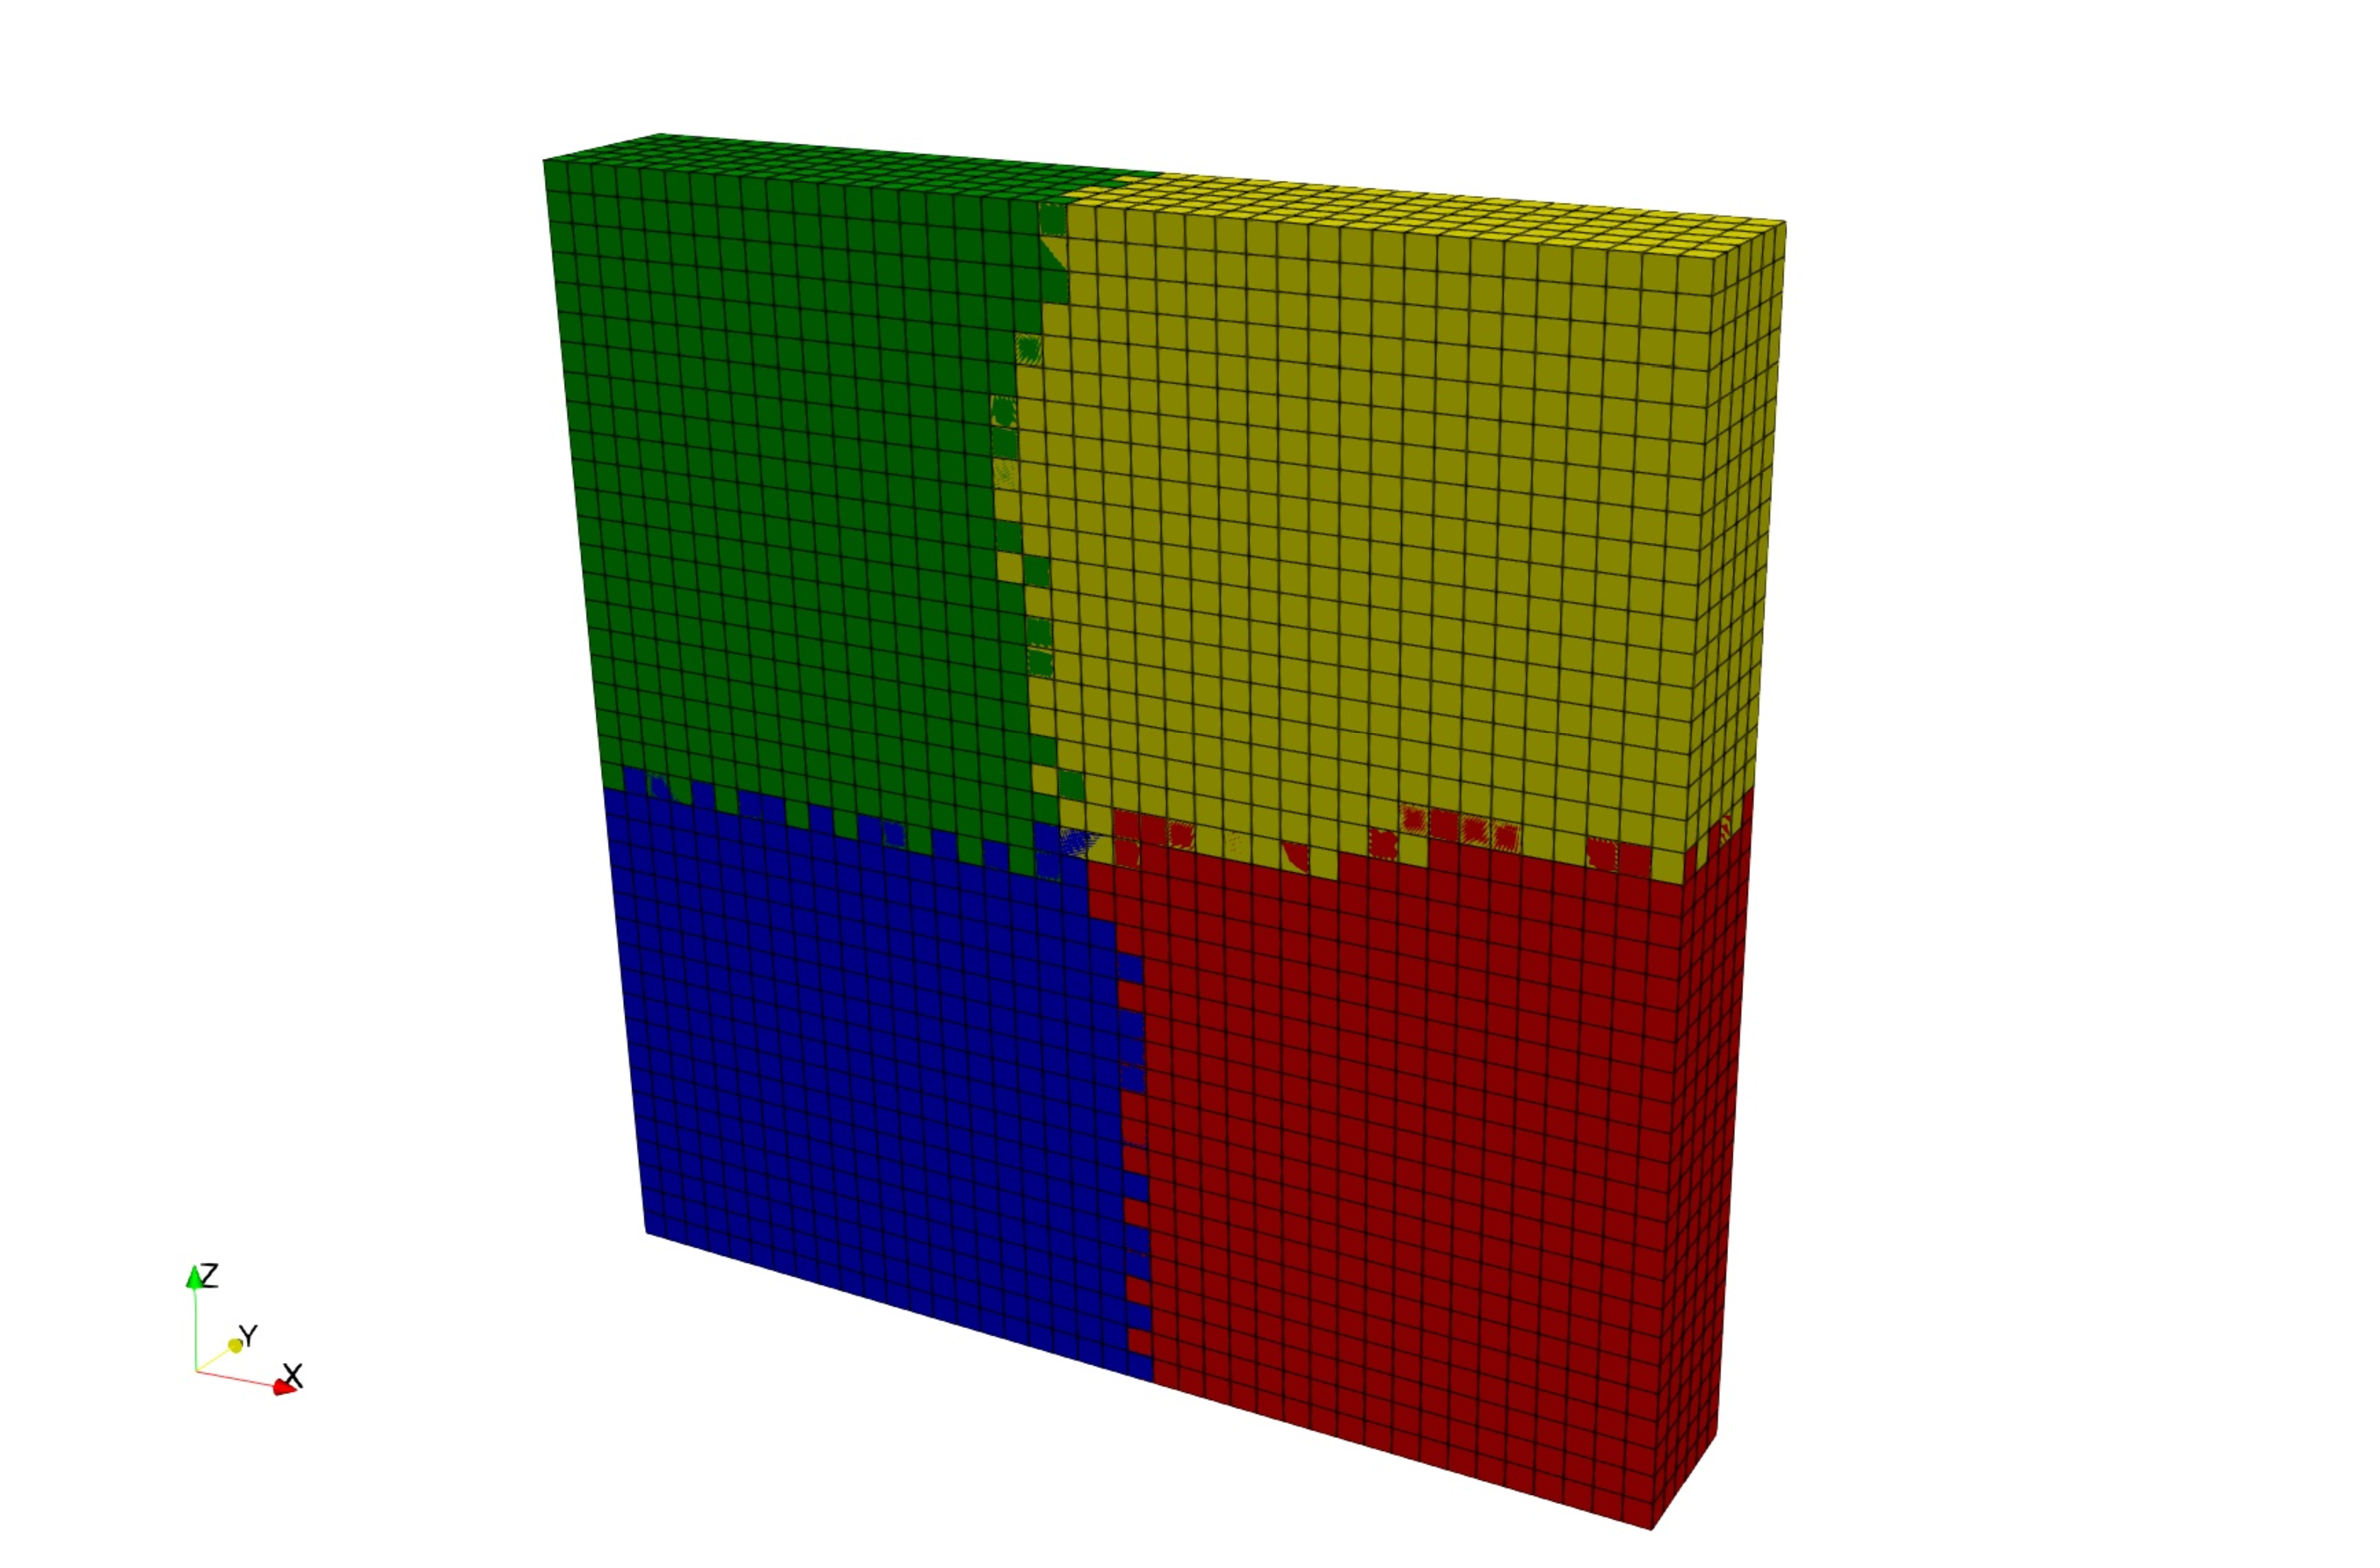
\includegraphics[width=10truecm]{pics/3d-dambreak-parallel/partition4.pdf}
	\caption{並列数4の場合の領域分割の図}
	\label{fig:3d-dambreak-parallel-partition}
\end{figure}


Figure \ref{fig:3d-dambreak-parallel-result}に速度分布、圧力分布、レベルセット関数の結果を示す。
並列化なしの場合と同様の結果が得られており、並列化解析が問題なくできていることが確認できた。
計算時間についても大幅に短くなっているが、時間計測は今回は行っていないため、今後スケーリング効果の計測を実施する。

\begin{figure}[H]
	\centering
	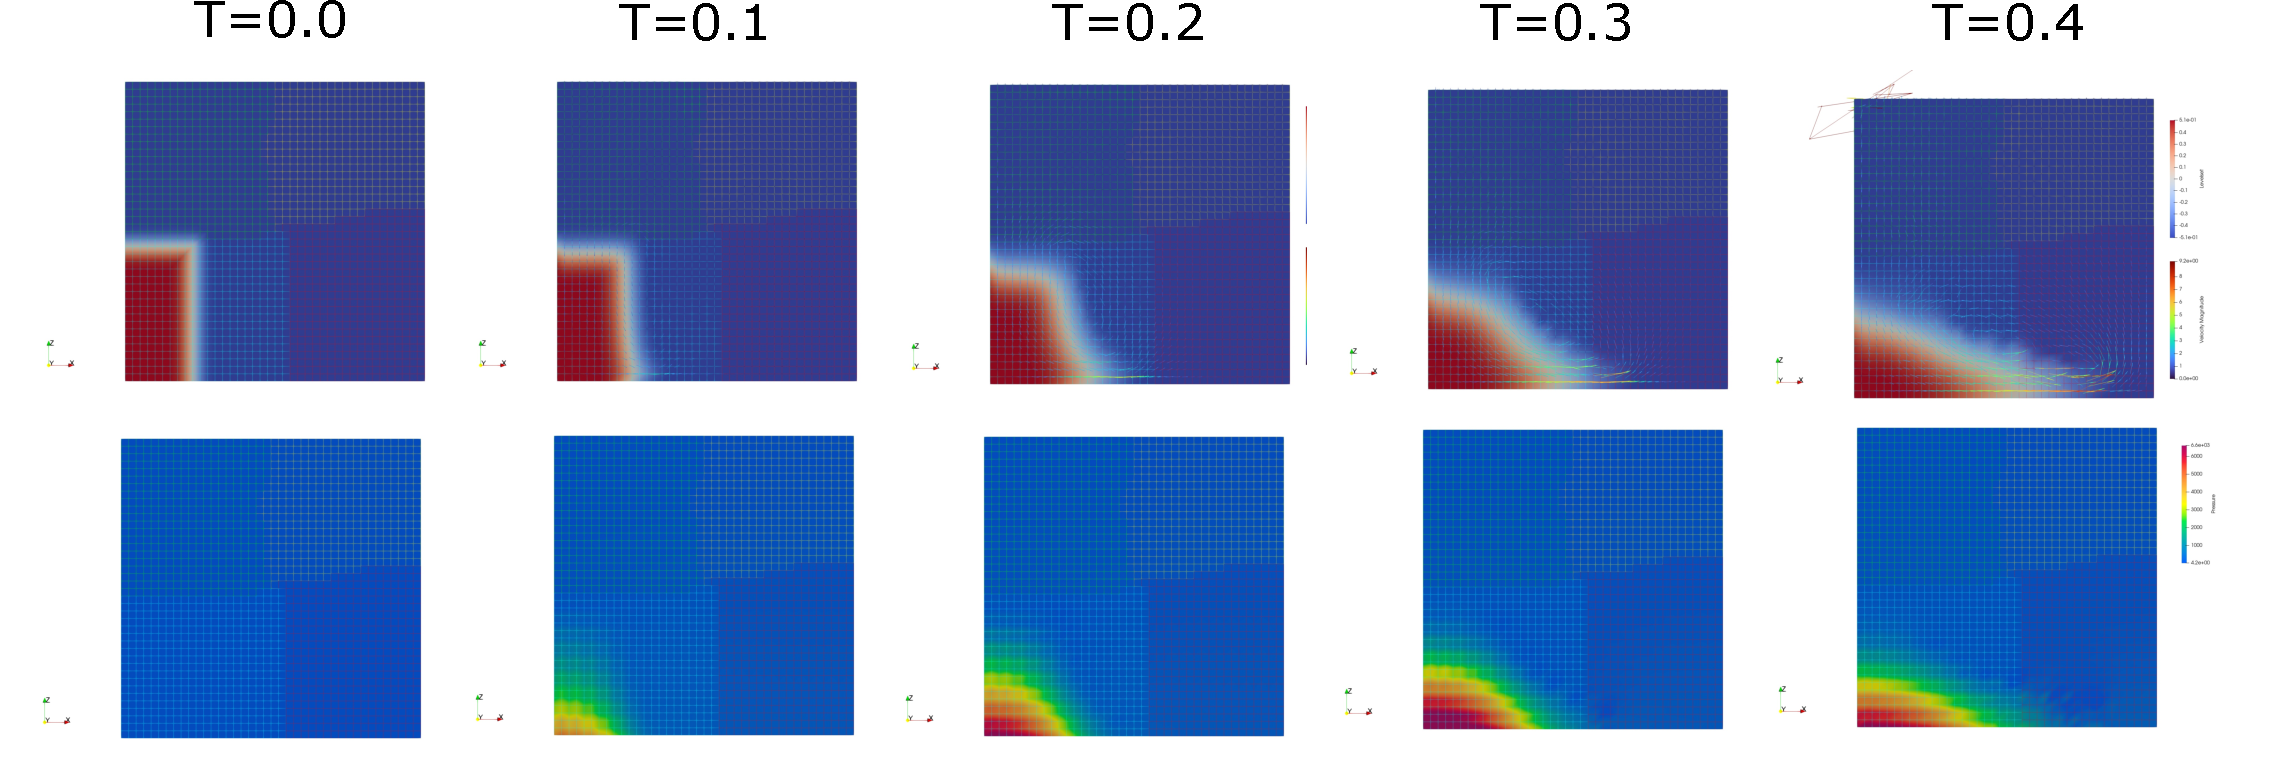
\includegraphics[width=18truecm]{pics/3d-dambreak-parallel/result-partition4.pdf}
	\caption{ダムブレイク問題のCase2の並列化解析による計算結果($y=0.4$における断面)。網目の色の違いで領域分割されている領域を可視化した。}
	\label{fig:3d-dambreak-parallel-result}
\end{figure}

ダムブレイクの検証\cite{Okumura2009}, 
有名な文献\cite{Koshizuka1996}
\end{comment}

\newpage
\subsection{解析結果(並列化計算)}

領域分割法による並列計算結果についても検証を行った。
図~\ref{fig:3d-dambreak-mesh-parallel16}に領域分割数16の場合の計算メッシュの分割結果を示す。
節点数は19683, 要素数は12800である。

\begin{figure}[H]
    \centering
    \includegraphics[width=6truecm]{pics/3d-dambreak-parallel/mesh_parallel16.jpeg}
	\caption{ダムブレイクの計算メッシュ(領域分割数16の場合)}
	\label{fig:3d-dambreak-mesh-parallel16}
\end{figure}

図~\ref{fig:3d-sloshing-result-parallel}に並列数2,4, 8, 16の場合の計算結果を示す。
並列数を変えた場合でも逐次計算の結果と一致した結果が得られた。

\begin{figure}[H]
    \centering
	\includegraphics[width=15truecm]{pics/3d-sloshing-parallel/sloshing_result_comparison_parallel.pdf}
	\caption{スロッシング解析結果の左端の水位と参考文献\cite{Okamoto1992}, \cite{Sakuraba2001}との比較}
	\label{fig:3d-sloshing-result-parallel}
\end{figure}